% Copyright 2004 by Till Tantau <tantau@users.sourceforge.net>.
%
% In principle, this file can be redistributed and/or modified under
% the terms of the GNU Public License, version 2.
%
% However, this file is supposed to be a template to be modified
% for your own needs. For this reason, if you use this file as a
% template and not specifically distribute it as part of a another
% package/program, I grant the extra permission to freely copy and
% modify this file as you see fit and even to delete this copyright
% notice. 

\documentclass{beamer}
\usepackage{algorithm,algorithmic}
\usepackage[croatian]{babel}
\makeatletter
\renewcommand*{\ALG@name}{Algoritam}
\makeatother
\setbeamertemplate{footline}[frame number]
\usepackage[utf8]{inputenc}
\newcommand\tab[1][1cm]{\hspace*{#1}}
% There are many different themes available for Beamer. A comprehensive
% list with examples is given here:
% http://deic.uab.es/~iblanes/beamer_gallery/index_by_theme.html
% You can uncomment the themes below if you would like to use a different
% one:
%\usetheme{AnnArbor}
%\usetheme{Antibes}
%\usetheme{Bergen}
%\usetheme{Berkeley}
%\usetheme{Berlin}
%\usetheme{Boadilla}
%\usetheme{boxes}
%\usetheme{CambridgeUS}
%\usetheme{Copenhagen}
%\usetheme{Darmstadt}
\usetheme{default}
%\usetheme{Frankfurt}
%\usetheme{Goettingen}
%\usetheme{Hannover}
%\usetheme{Ilmenau}
%\usetheme{JuanLesPins}
%\usetheme{Luebeck}
%\usetheme{Madrid}
%\usetheme{Malmoe}
%\usetheme{Marburg}
%\usetheme{Montpellier}
%\usetheme{PaloAlto}
%\usetheme{Pittsburgh}
%\usetheme{Rochester}
%\usetheme{Singapore}
%\usetheme{Szeged}
%\usetheme{Warsaw}

\usepackage{listings}
\usepackage[T1]{fontenc}
\lstset{
    literate=%
    {ć}{{\'c}}1
    {č}{{\v{c}}}1
    {đ}{{\dj{}}}1
    {š}{{\v{s}}}1
    {ž}{{\v{z}}}1
    {Ć}{{\'C}}1
    {Č}{{\v{C}}}1
    {Đ}{{\DJ{}}}1
    {Š}{{\v{S}}}1
    {Ž}{{\v{Z}}}1
}

\title{SVEUČILIŠTE U ZAGREBU \\ FAKULTET ELEKTROTEHNIKE I RAČUNARSTVA}

\author{ZAVRŠNI RAD br. 4573 \\ Obrada podataka tehnologijom Apache Spark}
  
\institute[Fakultet elektrotehnike i računarstva]{Martin Matak}% (optional, but mostly needed)
\date{Zagreb, srpanj 2016.}
% This is only inserted into the PDF information catalog. Can be left
% out. 

% If you have a file called "university-logo-filename.xxx", where xxx
% is a graphic format that can be processed by latex or pdflatex,
% resp., then you can add a logo as follows:

% \pgfdeclareimage[height=0.5cm]{university-logo}{university-logo-filename}
% \logo{\pgfuseimage{university-logo}}

% Delete this, if you do not want the table of contents to pop up at
% the beginning of each subsection:
\AtBeginSubsection[]
{
  \begin{frame}<beamer>{Sadržaj}
    \tableofcontents[currentsection,currentsubsection]
  \end{frame}
}

% Let's get started
\begin{document}

\begin{frame}
  \titlepage
\end{frame}

\begin{frame}{Sadržaj}
  \tableofcontents
  % You might wish to add the option [pausesections]
\end{frame}

% Section and subsections will appear in the presentation overview
% and table of contents.
\section{Uvod}
\begin{frame}{Uvod}
	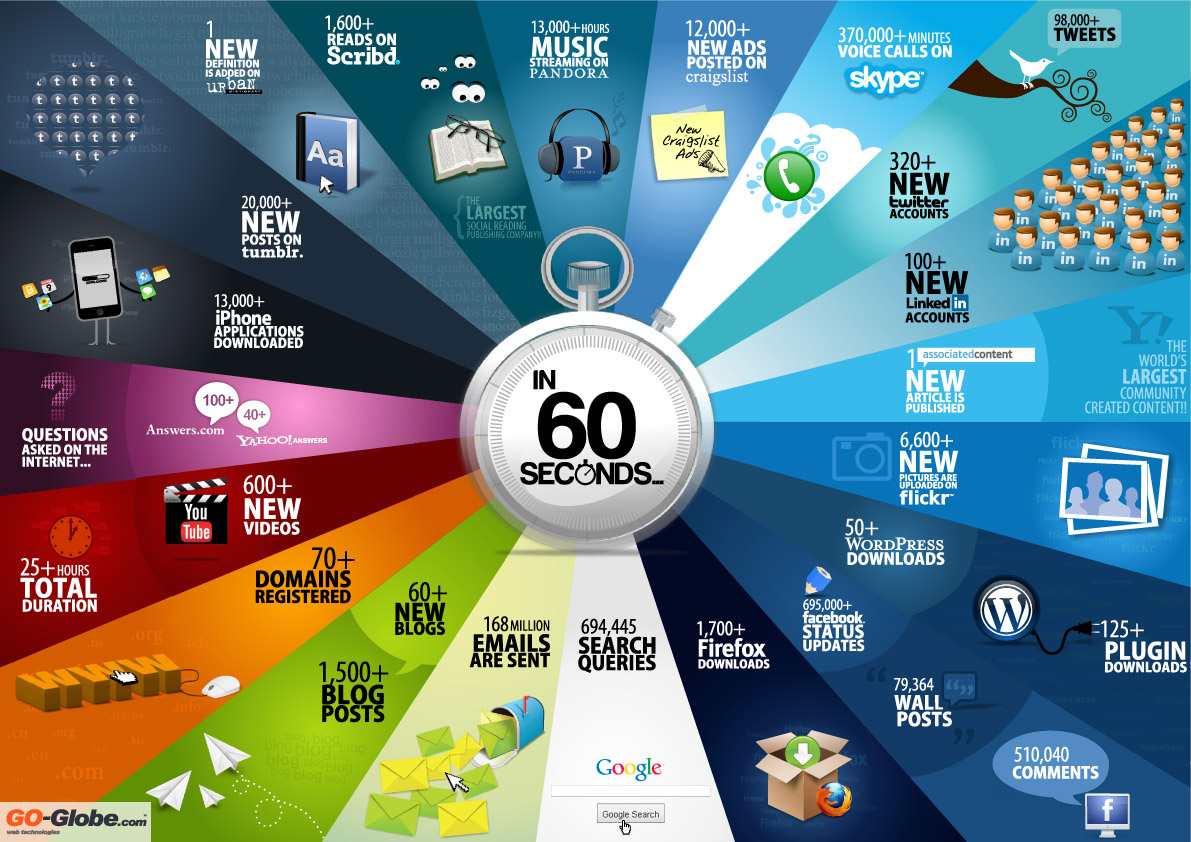
\includegraphics[width=300pt, height=180pt]{60seconds.jpg}%
\end{frame}

\section{Osnovni gradivni elementi}

\begin{frame}{Osnovni gradivni elementi}
	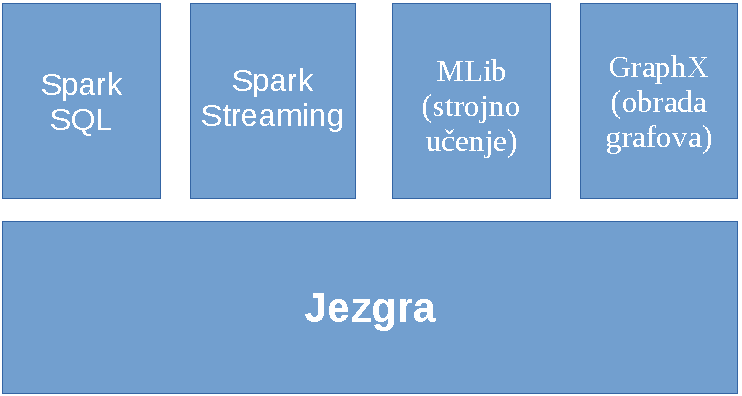
\includegraphics[width=300pt, height=180pt]{gradivniElementiCropped.pdf}%
\end{frame}

\section{Prvi programi}

\subsection{Postavljanje temelja}

\begin{frame}{Osnovni elementi aplikacije}
	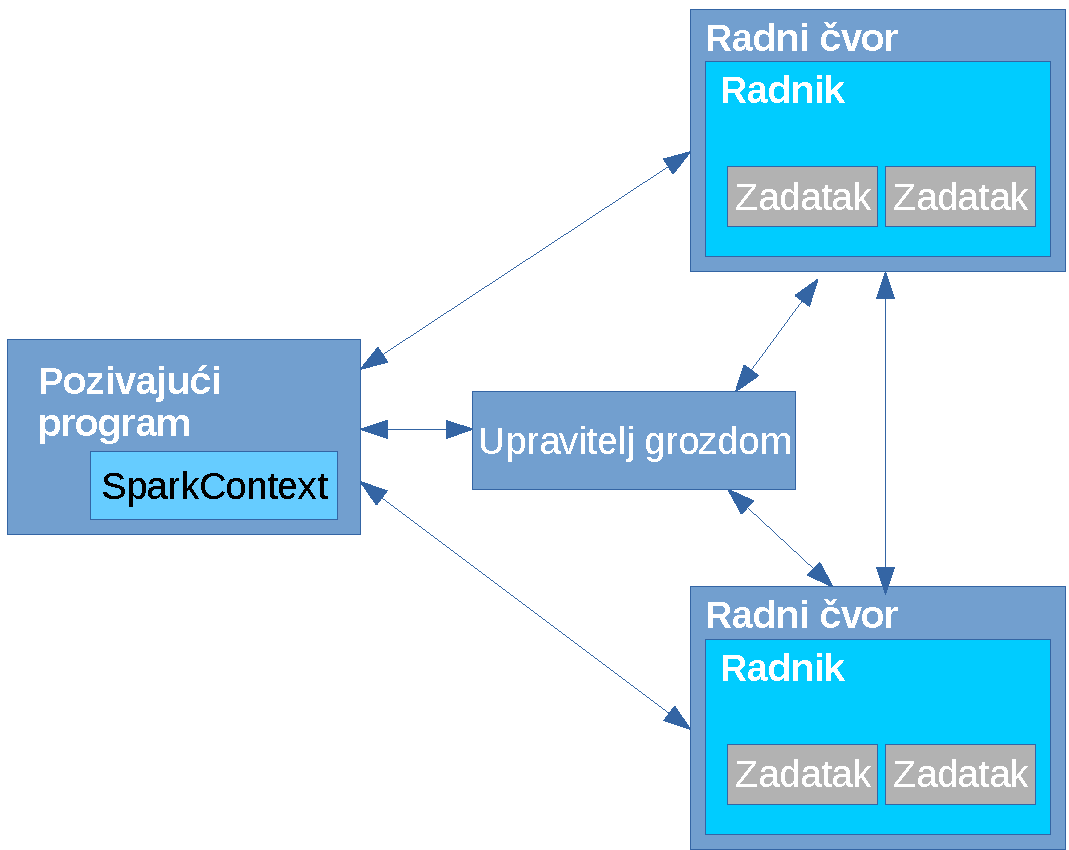
\includegraphics[width=300pt, height=180pt]{elementiAplikacijeCropped.pdf}%
\end{frame}

\subsection{Otporni rasopdijeljeni skup podataka}

\begin{frame}{Otporni raspodijeljeni skup podataka}{Resilient distributed dataset - RDD}
  \begin{itemize}
  \item {
 	Nepromjenjiva kolekcija podataka
 	\pause
  }
  
  \begin{block}{Transformacije}
	Operacije koje iz jednog skupa kreiraju drugi, novi skup podataka.
	\alert{Lijena evaluacija} - pokreću ih akcije.
	\end{block}  
	
  \pause
  \begin{block}{Akcije}
	Dohvat jednog ili više elemenata iz nekog skupa. 
  \end{block}
  \pause  
  
  \item {
 	Stanje u memoriji?
  }
  \end{itemize}
\end{frame}

\section{Napredno programiranje}
\subsection{Algoritam PageRank}
\begin{frame}{Koja stranica je najvažnija?}
	\begin{center}
		 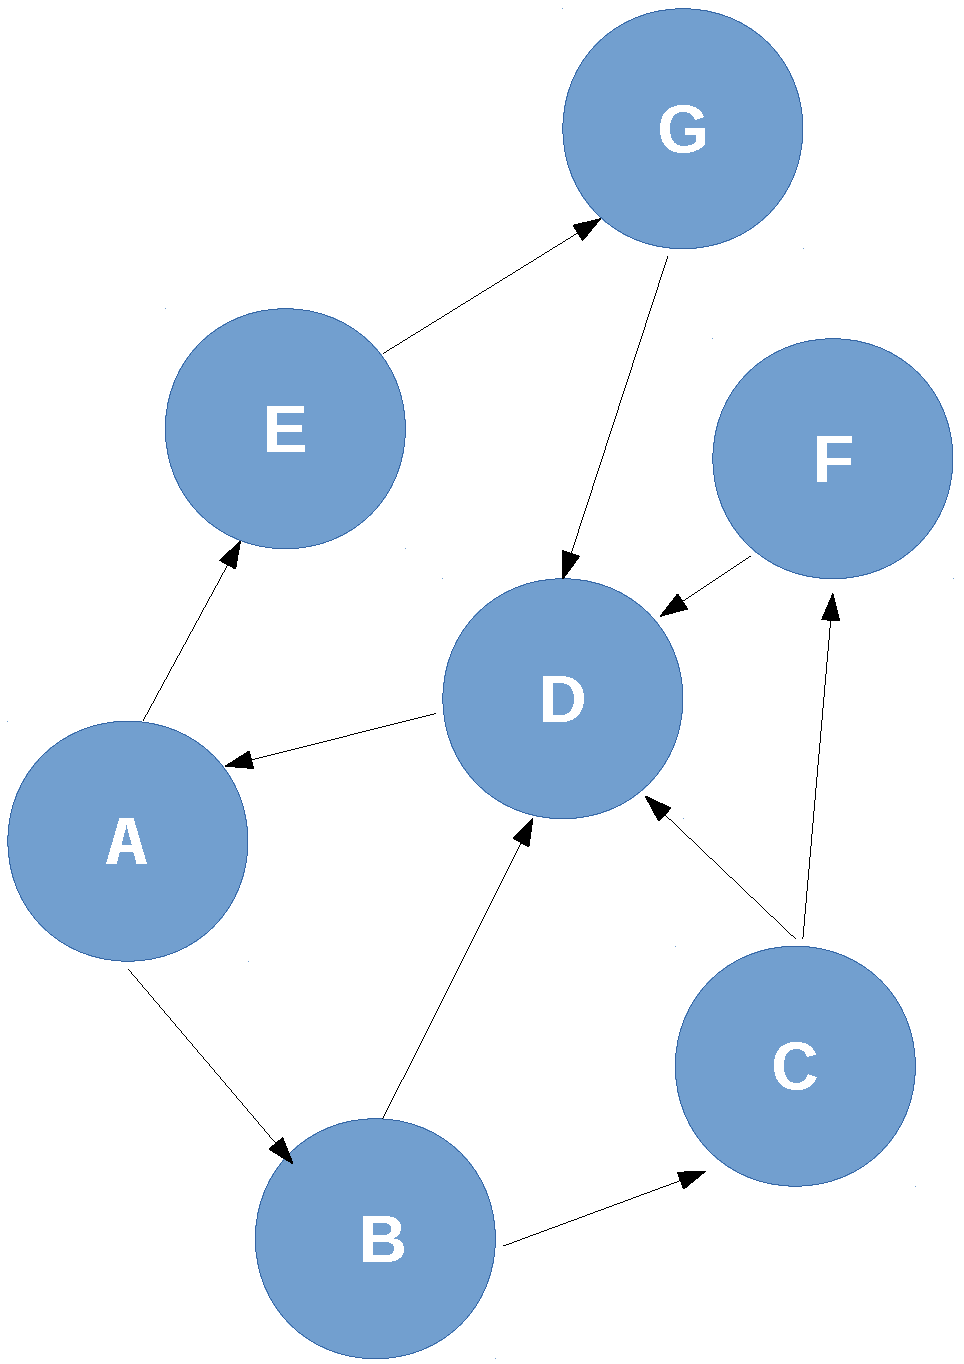
\includegraphics[width=200pt, height=180pt]{algoritamPageRankRucnoCropped.pdf}%
	\end{center}
\end{frame}

\begin{frame}{Algoritam PangeRank}
\begin{algorithm}[H]
\caption{Algoritam Pagerank}
\begin{algorithmic}[1]
\STATE{Početni rang svake stranice postavi se na $1.0$}
\FOR{$i=1$ to $P$}
\STATE{Svaka stranica \texttt{\textit{n}} šalje svojim susjedima doprinos\\
	\tab \texttt{rang(\textit{n})} / \texttt{brojSusjeda(\textit{n})}}
\STATE{Postavi ukupni rang stranice prema formuli: \\
	\tab $0.15 + 0.85 * $ \textit{ukupan primljeni doprinos}}
\ENDFOR
\end{algorithmic}
\end{algorithm}
\end{frame}

\begin{frame}{Rezultati}
\begin{center}
		 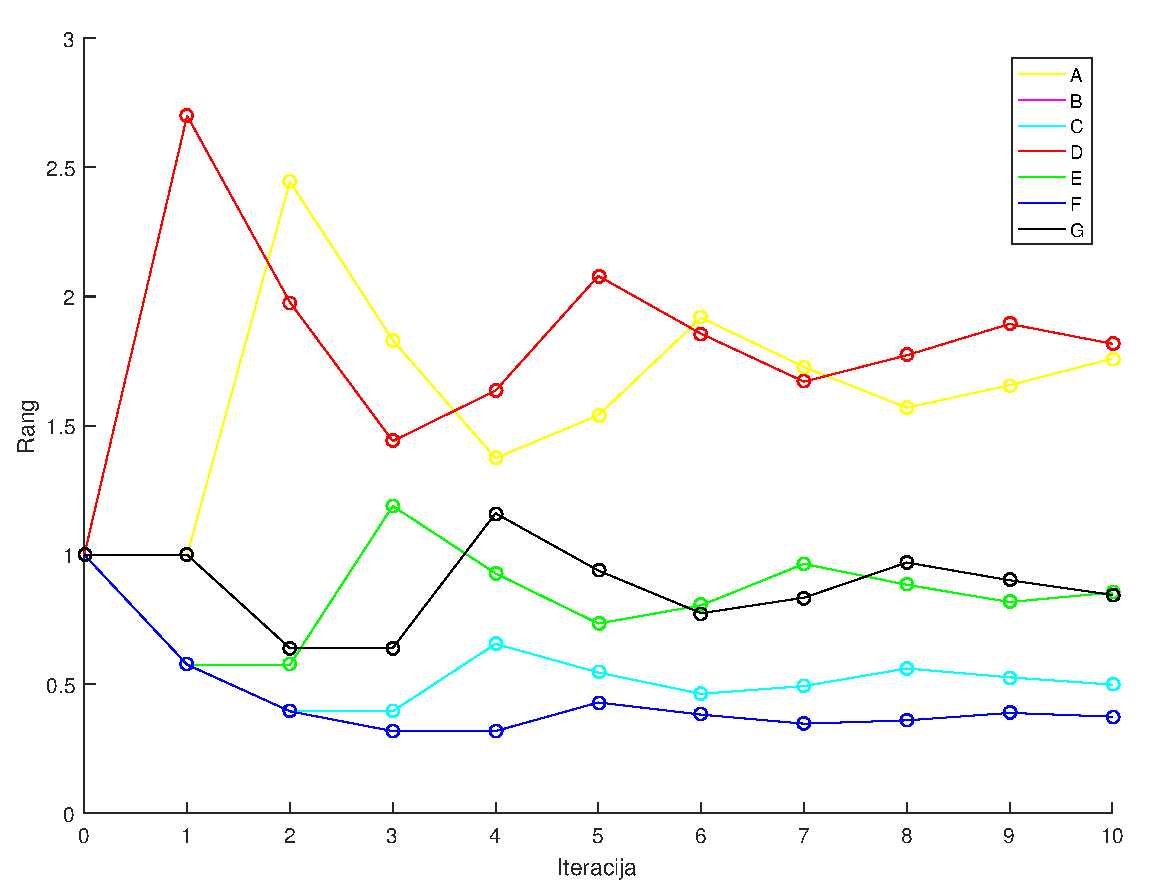
\includegraphics[width=300pt, height=200pt]{grafPageRankStraniceCropped.pdf}%
	\end{center}
\end{frame}

\subsection{Skupovi podataka kao uređeni parovi}
\begin{frame}{Uređeni parovi te spremanje i čitanje podataka}
  \begin{itemize}
  \item {
 	Podatci u obliku ključ - vrijednost
 	\pause
  }
  \item {
 	Posebne \textbf{transformacije} i \textbf{akcije}
 	\pause
  }
  \item {
 	Mogućnosti spremanja i čitanja: baze podataka, tekstualne datoteke (JSON, CSV, TSV) ...
  }  
  \end{itemize}
\end{frame}
\subsection{Dijeljene varijable}
\begin{frame}{Dijeljene varijable: odašiljatelji i akumulatori}
\begin{itemize}
  \item {
 	\alert{Problem: } Svaki zadatak na grozdu ima svoju kopiju varijabli
 	\pause
  }
\end{itemize}
\begin{block}{Odašiljatelj}
	Nepromjenjiva varijabla koja zauzima malo memorije čiju vrijednost je moguće dohvatiti na cijelom grozdu.
 \end{block}  
	
  \pause
  \begin{block}{Akumulator}
	Globalna varijabla čiju vrijednost je moguće mijenjati iz cijelog grozda.
  \end{block}
 \end{frame}
  
\section{U radu implementirano}
\begin{frame}{U radu implementirano}
\begin{itemize}
  \item {
 	Svi primjeri napisani su u Javi
 	\pause
  }
  \item {
 	Algoritam brojanja riječi - bez i s korištenjem lambda izraza
 	\pause
  }
  \item {
 	Primjer korištenja transformacija i akcija
 	\pause
  }
  \item {
 	Algoritam PageRank
 	\pause
  }
  \item {
 	Korištenje akumulatora za brojanje grešaka u \emph{log} datotekama
 	\pause
  }
  \item {
 	Korištenje odašiljatelja za dohvaćanje imena naselja pomoću identifikatora
 	\pause
  }
\end{itemize}
 \end{frame}
% Placing a * after \section means it will not show in the
% outline or table of contents.
\section{Zaključak}

\begin{frame}{Zaključak}
  \begin{itemize}
  \item
    Tehnologija za obradu velike količine podataka.
  \item
    Algoritam PageRank.
  \item
    Dijeljene varijable.
  \end{itemize}
  
  \begin{itemize}
  \item
    Još bi trebalo: 
    \begin{itemize}
    \item
      Postaviti i isprobati Apache Spark na grozdu.
    \item
      Razraditi svaku od komponenata - SparkSQL, MLib, Spark Streaming i GraphX.
    \end{itemize}
  \end{itemize}
\end{frame}

\end{document}


